%!TeX root = ../index.tex

\section{Schema Management}\label{sec:schema-management}

This section examines the problem domain of schema management by analyzing an example use case and parallel use cases from academic literature.
Before though, it provides essential information regarding the two prominent technologies of these use cases: Apache Kafka and Apache Avro.
Building on the analysis, the subsequent text deduces a definition of schema management and the characteristics of a schema management solution.

\subsection{Messaging Technologies}

\subsubsection{Apache Kafka}

The LinkedIn employees \citeauthor{kreps_kafka_2011} introduced their new \enquote{Event Streaming Platform} \emph{Kafka} in \citeyear{kreps_kafka_2011} \parencite{kreps_kafka_2011}.
Over a decade later, the project has since joined the Apache foundation and \enquote{[m]ore than 80\% of all Fortune 100 companies trust, and use [it]} \parencite{apache_software_foundation_apache_nodate}.

\citeauthor{kreps_kafka_2011} describe Kafka as \enquote{[\ldots] a novel messaging system for log processing [\ldots] that combines the benefits of traditional log aggregators and messaging systems.} \parencite{kreps_kafka_2011}.
The solution has an \gls{api} that is similar to traditional \gls{mom}, yet it persists messages in an append-only log structure on the hard drive.
This detail allows Kafka to not only stream data in near real-time but persist large amounts of it for online analytical processing.
In addition to that, Kafka features partitioning and replication mechanisms which make it highly available and scalable. \parencite{kreps_kafka_2011}

Kafka is not only useful for processing the kinds of log data that are proposed by \citeauthor{kreps_kafka_2011}: activity (e.~g. user logins, clicks, \enquote{likes}, \ldots) and operational data (e.~g. \gls{cpu} or disk utilization, \gls{http} requests, \ldots) \parencite{kreps_kafka_2011}.
\citeauthor{stopford_designing_2018}, for example, outlines how the entire state management and internal communication of a business application can be based on Apache Kafka.
His design implements concepts from the \gls{ddd} community like Event Sourcing \parencite{fowler_event_sourcing_2005} and \gls{cqrs} \parencite{fowler_cqrs_2011} with Apache Kafka's log-based messaging at the center \parencite{stopford_designing_2018}.
The potential use cases of Apache Kafka are therefore plentiful.

\subsubsection{Apache Avro}\label{sec:avro}

Apache Avro provides the ability to define rich data structures and interfaces for \glspl{rpc} as schema documents.
On top of that, it offers an efficient binary data format for serialization.
Listing \ref{lst:avro-schema-person} shows an example for an Avro schema describing a customer entity.
\parencite{apache_software_foundation_apache_2021}

\begin{listing}[H]
  \inputminted{json}{assets/src/Customer.avsc}
  \caption{Simplified Avro Schema of a Customer Entity}\label{lst:avro-schema-person}
\end{listing}

Avro's design assumes that applications which (de)-serialize data have access to the data's schema.
That is one of the reasons why the format is so efficient.
It does not need to include type information in the serialized data.
Avro's support for schema evolution builds upon this assumption.
If an application attempts to de-serialize data encoded in Avro binary, it requires both the schema with which the data was written and the schema which the application understands.
These schemas are called the \emph{writer} and the \emph{reader} schema respectively.
In the simplest case, these schemas might be equal.
Nevertheless, Avro also supports de-serializing data with a reader schema different from the writer schema.
Although, the de-serialization will only succeed if both schemas are still \emph{compatible}.
\parencite{apache_software_foundation_apache_2021}

If, for example, the reader schema had an additional field without a default value.
It would be an incompatible change because Avro would not be able to infer a value for the additional field.
On the other hand, if the field had a default value, the de-serialization would succeed.
\citeauthor{kreps_kafka_2011} chose Apache Avro as the serialization protocol for their message payloads due to its efficiency and schema evolution capabilities \parencite{kreps_kafka_2011}. 

\subsection{The Case for Schema Management}

This section examines the problem domain that schema management addresses.
It does so by analyzing the hypothetical \gls{is} design for a web-shop application depicted in figure \ref{fig:web-shop}.
The analysis serves as a basis for a definition of schema management and the characteristics of schema management solutions.

\begin{figure}[H]
  \centering
  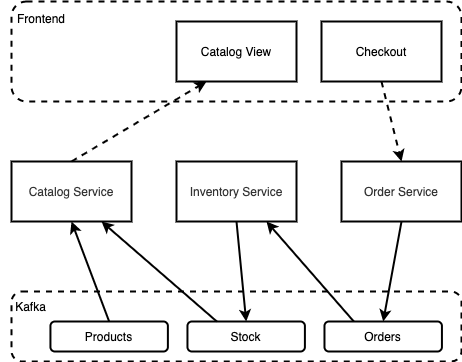
\includegraphics[width=0.8\linewidth]{webshop.drawio.png}
  \caption{Simplified Web-Shop Design Using Apache Kafka}\label{fig:web-shop}
\end{figure}

The design is loosely based on a design proposed in \cite[p.~148]{stopford_designing_2018} but condensed for simplicity.
The boxes in the \enquote{Frontend} section depict fragments of the shop's \gls{ui}, and the dashed arrows signify synchronous, \gls{http}-based communication.
Further down, the three boxes each represent a microservice.

\begin{description}
  \item[Catalog Service] Presents a view of the currently available products and their current stock.
  \item[Inventory Service] Keeps track of the shop's inventory and updates the stock based on incoming orders.
  \item[Order Service] Handles users' order requests from the Checkout.
\end{description}

All of these services communicate amongst each other via messages that they write to or read from Kafka topics.\todo{explain kafka topics}
The plain arrows depict the producing and consuming of messages.
A typical ordering process could look like this:

\begin{enumerate}
  \item The Catalog Service consumes messages from the Products and Stock topics to calculate a view of the shop's current stock, enhanced with product details.
  \item A user visits the shop and the Catalog View requests the current stock from the Catalog Service.
  \item The user adds a product to their shopping cart and proceeds to the Checkout.
  \item The Checkout sends a request to the Order Service to complete the user's order.
  \item The Order Service creates the order (checks the successful payment, sends an email, \ldots) and publishes an \texttt{OrderCreated} event as a message to the Orders topic.
  Listing \ref{lst:order-created} in the appendix shows what the schema for an \texttt{OrderCreated} event might look like.
  \item This new event is consumed by the Inventory Service. It updates the stock accordingly by publishing a \texttt{StockUpdated} event to the Stock topic.
  \item The Catalog Service consumes the new event and updates its view of the current stock.
\end{enumerate}

Furthermore, the design uses Apache Avro for the following purposes:

\begin{itemize}
  \item Efficient data transfer and storage by serializing message payloads in Avro's compact binary format.
  \item Improved interoperability by using schemas as communication contracts.
  \item Improved flexibility via schema evolution. In other words, it allows compatible changes to message schemas without breaking the contract.
\end{itemize}

Using schemas also creates new problems.
A system that uses schemas for its communication needs to distribute them to all communicating parties---meaning applications---at both the compile-time and the run-time.
The following paragraphs explain why that is and what possible solutions exist.

% If multiple services need to work with an event of the same type, then both require the message schema of that event.
% For example, this is the case for the Order Service and the Inventory Service.
% They both produce or consume messages of the type \texttt{OrderCreated}, so they both need to have the schema for this message type.

Each application requires the schema of a message type that it wants to work with at its compilation.
Otherwise, if the application wants to produce a message, it would not know how to serialize the payload.
If it wants to consume a message, it would not know how to interpret its structure.

A simple solution is to package the schemas using a dependency management tool.
For Java-based projects, for example, they could be packaged into a Maven\footnote{\url{https://maven.apache.org/}} Artifact and published to a registry.
The individual services could then declare this artifact as a dependency to include the schemas during their compilation.
This solution comes with the caveat that the package would be language-dependent.
To consume the schemas in a NodeJS-based application, they also need to be packaged and published as an artifact of NodeJS' package management tool NPM.
These factors create overhead and a potentially complicated setup for \gls{cicd}.
Additionally, it requires all of the projects which consume the message schema dependency to upgrade it manually if they want to use the most recent schemas.

Beyond the disadvantages of the described solution, it fulfills the requirement of distributing schemas at compile-time.
By distributing schemas at compile-time, the system benefits from the efficiency of Avro's binary format.
It also creates a weak communication contract between producers and consumers.
Consumers can check if the payloads that they de-serialize match the schemas they expect and reject those that do not.
However, no check exists on the producer side, meaning they can write incompatible data to the topic.
Still, if the system is supposed to harness the full advantages of schemas, they also need to be distributed amongst the applications at run-time.

As described in \ref{sec:avro}, Avro supports schema evolution by allowing some differences between the schema used to serialize data and the schema used to de-serialize that data.
This schema evolution can make the application more flexible by reducing the coupling between the microservices.
If consumers had access to all versions of schemas they are interested in, they could handle one-sided changes to those schemas.

Consider this scenario: The Order Service adds a field with a default value to the schema of \texttt{OrderCreated} events---a compatible change---and is deployed.
With \emph{only compile-time distribution} of schemas, the Inventory Service would not be able to consume the messages produced by this new version of the \texttt{OrderService}.
That is because the Inventory Service only knows a single version of the schema for \texttt{OrderCreated} events, which does not match the writer schema of the new messages.
This breaks the communication between the two microservices.
To fix it again, the developers must upgrade the version of the schema used by the Inventory Service and deploy it anew.
The rigid dependency on shared schemas creates tight coupling between the Inventory Service and the Order service.

With \emph{run-time distribution} of schemas, the Inventory Service can access the specific version of a message's schema dynamically at run-time.
Therefore, if the Order service sends \texttt{OrderCreated} events with a new version of the message schema, the Inventory service can download this new version when consuming the messages.
That means that both the writer and reader schema are present at de-serialization, allowing Avro to map between them and produce the data in a format the service can use.
Run-time distribution allows producers to change their message schemas without breaking communication.
Therefore, it loosens the coupling between the services and makes the application more flexible.

One question remains: How are schemas provided to services at run-time?
That is where schema management solutions come into the picture.



% A simple solution is to include the message schema in the message's headers\todo{explain message structure}.
% This way, only the application which writes messages of a certain type needs 
% Although this would diminish the efficiency advantage of Avro's binary format, which is in part achieved by \emph{not} including the schema with the serialized payload.

% Therefore, the system needs to distribute the schemas to the applications in another way.


% It features a set of microservice applications hosted on virtualized infrastructure and employs Apache Kafka as a \gls{mom} to facilitate the communication between the microservices.
% Cross-functional teams develop and deploy each microservice with a great degree of independence.
% The teams use Apache Avro to define schemas for the messages that the microservices send and receive.
% They have integrated it into the services to serialize the payload of a message into Avro's binary format before they send it to Kafka.


\subsection{Definition of Schema Management}

\subsection{Characteristics of Schema Management Solutions}
